\chapter{संक्रमण धातुएँ और उपसहसंयोजन संकुल}\label{ch:b2:coordination-complexes}

1893 में छब्बीस वर्ष के एक रसायनज्ञ, आल्फ़्रेड वर्नर, ने एक पहेली सुलझाने का बीड़ा उठाया।
कोबाल्ट(III) क्लोराइड अमोनिया के साथ चार यौगिक बनाता है, \ce{CoCl3.6NH3},
\ce{CoCl3.5NH3} और सूत्र \ce{CoCl3.4NH3} वाले दो, एक हरा और एक बैंगनी।
सिल्वर नाइट्रेट पहले यौगिक के तीनों क्लोराइड तुरंत अवक्षेपित कर देता है, दूसरे के
दो, और अंतिम दोनों में से हर एक का केवल एक। वर्नर का उत्तर --- धातु के चारों ओर
एक अष्टफलक के कोनों पर छह समूह बँधे हैं, शेष बाहर
--- उपसहसंयोजन रसायन की नींव बना। यह अध्याय प्रथम वर्ष के खंड के संकुलों को
उनकी ज्यामिति, उनके समावयवियों, उनके नामों, और इलेक्ट्रॉनों की उस गिनती तक ले जाता है जो
बताती है कि कौन-से धातु कार्बोनिल अस्तित्व में हैं।

\begin{recall}
प्रथम वर्ष का खंड: संकुल, केंद्रीय परमाणु, लिगैंड, बहुदंतुर लिगैंड, कीलेट,
संभवन स्थिरांक, उपसहसंयोजन संख्या; संक्रमण धातु आयनों के इलेक्ट्रॉनिक विन्यास
($n$s इलेक्ट्रॉन पहले खोए जाते हैं); लुइस अम्ल और क्षारक,
उपसहसंयोजी आबंध; VSEPR; ऑक्सीकरण संख्याएँ; प्रतिबिंबरूप। \Cref{ch:b2:atomic-orbitals}:
d कक्षक और 4s तथा 3d स्तरों का क्रम।
\end{recall}

\begin{omfigure}
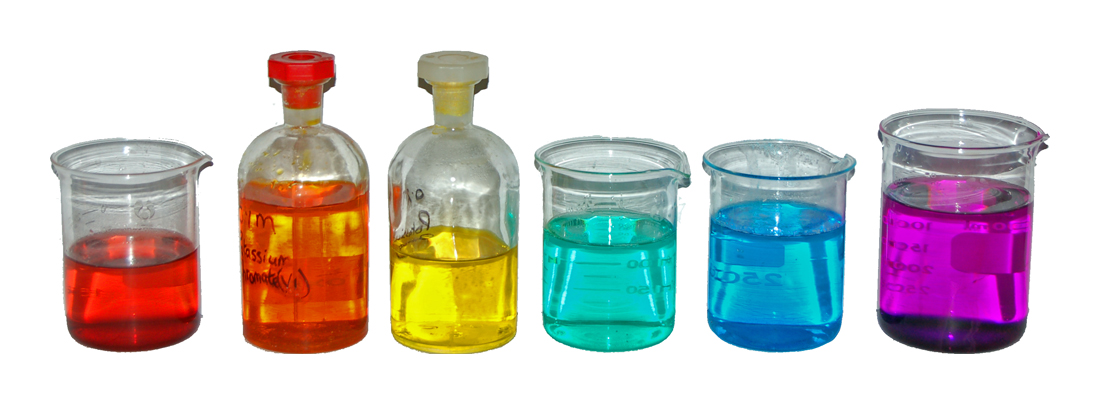
\includegraphics[width=0.8\linewidth]{images/book3/tm-solutions.jpg}

{\small संक्रमण धातु यौगिकों के जलीय विलयन: बाएँ से दाएँ,
कोबाल्ट(II) नाइट्रेट, पोटैशियम डाइक्रोमेट, पोटैशियम क्रोमेट, निकेल(II) क्लोराइड,
कॉपर(II) सल्फ़ेट और पोटैशियम परमैंगनेट। कोबाल्ट, निकेल
और कॉपर के विलयनों के रंग उनके ऐक्वा संकुलों से आते हैं। (छायाचित्र: बेंजा-बीएमएम27,
सार्वजनिक अधिकार-क्षेत्र, विकिमीडिया कॉमन्स।)}
\end{omfigure}

\section{d खंड}

\begin{definition}[संक्रमण तत्व]\label{def:b2:coordination-complexes:transition-element}
\emph{संक्रमण तत्व}\index{संक्रमण तत्व} वह तत्व है जिसके परमाणु में, या
जिसके किसी सामान्य आयन में, आंशिक रूप से भरा d उपकोश हो। ऐसे तत्व का कोई आयन
जिसके d कक्षकों में $n$ इलेक्ट्रॉन हों, \emph{$d^n$ विन्यास}\index{dn विन्यास@$d^n$ विन्यास} रखता है।
\end{definition}

\begin{proposition}[d इलेक्ट्रॉनों की गिनती]\label{prop:b2:coordination-complexes:dn}
कोई संक्रमण धातु आयन $\mathrm M^{m+}$, जो समूह संख्या $g$ (3 से 12) का हो,
$d^n$ विन्यास रखता है, जहाँ $n = g - m$।
\end{proposition}

\begin{proof}
उदासीन परमाणु के पिछली उत्कृष्ट गैस से आगे $g$ इलेक्ट्रॉन हैं, जो $n$s और
$(n - 1)$d कक्षकों में हैं। आयनों में d कक्षक s कक्षक से नीचे होते हैं
(\cref{ex:b2:atomic-orbitals:iron}): शेष सभी $g - m$ संयोजकता इलेक्ट्रॉन d
इलेक्ट्रॉन हैं।
\end{proof}

उदाहरण के लिए \ce{Fe^2+} (समूह 8) $d^6$ है, \ce{Cu^2+} (समूह 11) $d^9$, \ce{Co^3+} (समूह 9)
$d^6$, \ce{Pt^2+} (समूह 10) $d^8$।

\section{लिगैंड}

\begin{definition}[दंतुरता]\label{def:b2:coordination-complexes:denticity}
किसी लिगैंड की \emph{दंतुरता}\index{दंतुरता} उसके उन परमाणुओं की संख्या है जो
एक ही केंद्रीय परमाणु से बँधे हों। \emph{एकदंतुर लिगैंड}\index{एकदंतुर लिगैंड}
एक परमाणु से बँधता है (\ce{H2O}, \ce{NH3}, \ce{Cl-}, \ce{CO}), \emph{द्विदंतुर
लिगैंड}\index{द्विदंतुर लिगैंड} दो से (एथेन-1,2-डाइऐमीन, जिसे en लिखा जाता है;
एथेनडाइओएट आयन, ox)। \emph{सेतु लिगैंड}\index{सेतु लिगैंड} एक साथ दो
धातु परमाणुओं से बँधता है। \emph{उभयदंतुर लिगैंड}\index{उभयदंतुर लिगैंड}
दो भिन्न परमाणुओं में से किसी एक से बँध सकता है, जैसे नाइट्राइट आयन (N या O से) या
थायोसायनेट (S या N से)।
\end{definition}

\begin{definition}[उपसहसंयोजन मंडल]\label{def:b2:coordination-complexes:coordination-sphere}
किसी संकुल का \emph{उपसहसंयोजन मंडल}\index{उपसहसंयोजन मंडल} केंद्रीय परमाणु
और उससे बँधे लिगैंडों का समुच्चय है, जिसे वर्ग कोष्ठकों में लिखा जाता है; कोष्ठकों के
बाहर के आयन प्रति-आयन हैं, धातु से बँधे नहीं।
\end{definition}

\begin{omfigure}
\setchemfig{atom sep=2.2em}
\chemfig{M*5(-H_2N-CH_2-CH_2-NH_2-)}
\qquad
\chemfig{M*5(-O-(=O)-(=O)-O-)}
\qquad
\chemfig{N(-[:120]CH_2COO^{-})(-[:240]CH_2COO^{-})-CH_2-CH_2-N(-[:60]CH_2COO^{-})(-[:-60]CH_2COO^{-})}

\medskip
{\small कीलेटी लिगैंड। बाएँ: एथेन-1,2-डाइऐमीन (en), अपने दोनों
नाइट्रोजनों से द्विदंतुर। मध्य: एथेनडाइओएट आयन (ox), दो ऑक्सीजनों से द्विदंतुर। दाएँ:
ईडीटीए ऋणायन, जो अपने दोनों नाइट्रोजनों और चार
कार्बॉक्सिलेट ऑक्सीजनों से किसी धातु आयन को लपेट लेता है (षड्दंतुर)।}
\end{omfigure}

\section{उपसहसंयोजन संख्याएँ और ज्यामितियाँ}

दो, चार और छह सबसे सामान्य उपसहसंयोजन संख्याएँ हैं। सिल्वर(I) और गोल्ड(I)
रैखिक संकुल देते हैं (\ce{[Ag(NH3)2]+}); चार लिगैंड एक चतुष्फलक बनाते हैं
(\ce{[CoCl4]^2-}, \ce{[Zn(NH3)4]^2+}) या एक वर्ग (\ce{[PtCl4]^2-}, \ce{[Ni(CN)4]^2-});
पाँच, एक त्रिकोणीय द्विपिरामिड (\ce{Fe(CO)5}); छह, जो कहीं सबसे अधिक बार मिलता है, एक
अष्टफलक।

\begin{omfigure}
\begin{tikzpicture}[font=\small]
  \node[omligand] at (-0.8,0) {}; \node[omligand] at (0.8,0) {};
  \draw[thick, black!70] (-0.8,0) -- (0.8,0); \node[ommetal] at (0,0) {};
  \node at (0,-1.5) {रैखिक, 2};
  \pic at (3,0) {omtetrahedron}; \node at (3,-1.5) {चतुष्फलकीय, 4};
  \pic at (6,0) {omsquareplanar}; \node at (6,-1.5) {वर्ग समतलीय, 4};
  \pic at (9,0) {omtbp}; \node[align=center] at (9,-1.65) {त्रिकोणीय\\ द्विपिरामिडी, 5};
  \pic at (12,0) {omoctahedron}; \node at (12,-1.5) {अष्टफलकीय, 6};
\end{tikzpicture}

{\small सामान्य उपसहसंयोजन ज्यामितियाँ (धातु नारंगी, लिगैंड धूसर; खंडित
आबंध पृष्ठ के पीछे की ओर इंगित करते हैं)।}
\end{omfigure}

VSEPR, जो केंद्रीय परमाणु के इलेक्ट्रॉन युग्मों को एक-दूसरे से यथासंभव दूर रखता है,
यहाँ विफल होता है: \ce{Pt^2+} जैसा कोई $d^8$ आयन d इलेक्ट्रॉनों के चार युग्म और चार
लिगैंड रखता है, फिर भी उसके संकुल वर्गाकार हैं, न चतुष्फलकीय, न अष्टफलकीय।
d इलेक्ट्रॉन लिगैंडों को धकेलने वाले स्थानीकृत युग्म नहीं हैं: उनकी ऊर्जाएँ
ज्यामिति पर उस ढंग से निर्भर करती हैं जिसे अगला अध्याय परिकलित करता है।

\begin{proposition}[वर्ग समतलीय $d^8$]\label{prop:b2:coordination-complexes:square-planar}
दूसरी और तीसरी संक्रमण श्रेणियों के $d^8$ आयनों (\ce{Pd^2+}, \ce{Pt^2+}, \ce{Au^3+}) के
चतुःउपसहसंयोजी संकुल वर्ग समतलीय होते हैं।
\end{proposition}

\admitted

इसकी व्याख्या, लिगैंडों द्वारा d स्तरों का विपाटन, \cref{ch:b2:ligand-field}
में आती है।

\section{समावयवी}

\begin{definition}[संकुलों के समावयवी]\label{def:b2:coordination-complexes:isomers}
किसी अष्टफलकीय संकुल $\mathrm{MA_3B_3}$ में \emph{फ़ैक समावयवी}\index{फ़ैक समावयवी} के
तीनों B लिगैंड अष्टफलक के एक फलक पर होते हैं, \emph{मेर
समावयवी}\index{मेर समावयवी} के एक याम्योत्तर पर (धातु से होकर जाने वाले एक तल में
तीन स्थितियाँ)। \emph{बंधनी समावयवी}\index{बंधनी समावयवी} उस परमाणु में भिन्न होते हैं जिससे
कोई \omterm{def:b2:coordination-complexes:denticity}{उभयदंतुर लिगैंड} बँधता है। \emph{आयनन समावयवी}\index{आयनन समावयवी}
किसी लिगैंड का किसी प्रति-आयन से आदान-प्रदान करते हैं, जिससे विलयन में भिन्न आयन मिलते हैं।
\end{definition}

\begin{proposition}[अष्टफलकीय समावयवियों की गिनती]\label{prop:b2:coordination-complexes:isomer-count}
अष्टफलक में $\mathrm{MA_4B_2}$ के दो समावयवी हैं (cis और trans), $\mathrm{MA_3B_3}$ के दो
(फ़ैक और मेर), और तीन \omterm{def:b2:coordination-complexes:denticity}{द्विदंतुर लिगैंडों} वाले $\mathrm M(\mathrm{AA})_3$ के दो
प्रतिबिंबरूप, $\Delta$ और $\Lambda$।
\end{proposition}

\begin{proof}
अष्टफलक में कोई भी दो स्थितियाँ या तो सन्निकट होती हैं (cis, $90^\circ$) या आमने-सामने
(trans, $180^\circ$): दोनों B लिगैंडों के लिए दो व्यवस्थाएँ। तीन B लिगैंडों के लिए
या तो कोई दो trans नहीं होते (वे एक फलक घेरते हैं: फ़ैक) या ठीक एक युग्म trans होता है (तीसरा
दोनों के cis होता है: मेर); तीन परस्पर trans स्थितियाँ होती ही नहीं।
$\mathrm M(\mathrm{AA})_3$ के लिए हर कीलेट दो cis स्थितियों को फैलाता है; तीनों कीलेट
त्रिक अक्ष के परितः किसी प्रोपेलर के फलकों की तरह लिपटते हैं, उस अक्ष के अनुदिश देखने पर
या तो दक्षिणावर्त घूमते हुए या वामावर्त: दो दर्पण प्रतिबिंब, जो अध्यारोपणीय नहीं हैं
क्योंकि संकुल का कोई दर्पण तल नहीं है।
\end{proof}

\begin{omfigure}
\begin{tikzpicture}[font=\scriptsize]
  \pic (a) at (0,0) {omoctahedron};
  \node[omligand, fill=omDef!70] at (a-L1) {}; \node[omligand, fill=omDef!70] at (a-L3) {};
  \node at (0,-1.5) {\small cis-$\mathrm{MA_4B_2}$};
  \pic (b) at (3,0) {omoctahedron};
  \node[omligand, fill=omDef!70] at (b-L1) {}; \node[omligand, fill=omDef!70] at (b-L2) {};
  \node at (3,-1.5) {\small trans-$\mathrm{MA_4B_2}$};
  \pic (c) at (6.5,0) {omoctahedron};
  \node[omligand, fill=omThm!70] at (c-L1) {}; \node[omligand, fill=omThm!70] at (c-L3) {}; \node[omligand, fill=omThm!70] at (c-L5) {};
  \node at (6.5,-1.5) {\small फ़ैक-$\mathrm{MA_3B_3}$};
  \pic (d) at (9.5,0) {omoctahedron};
  \node[omligand, fill=omThm!70] at (d-L1) {}; \node[omligand, fill=omThm!70] at (d-L2) {}; \node[omligand, fill=omThm!70] at (d-L3) {};
  \node at (9.5,-1.5) {\small मेर-$\mathrm{MA_3B_3}$};
\end{tikzpicture}

\medskip
\begin{tikzpicture}[font=\scriptsize]
  \foreach \xs/\s/\lab in {0/1/{$\Delta$}, 4.5/-1/{$\Lambda$}} {
    \begin{scope}[xshift=\xs cm, xscale=\s]
      \draw[black!30] (0,0) circle (1.2);
      \foreach \a in {90, 210, 330} {
        \coordinate (p) at (\a:1.1); \coordinate (q) at (\a+70:0.55);
        \draw[very thick, omDef] (\a:1.1) .. controls (\a+30:1.25) and (\a+60:0.9) .. (\a+75:0.55);
        \node[omligand] at (\a:1.1) {}; \node[omligand] at (\a+75:0.55) {};
      }
      \node[ommetal] at (0,0) {};
    \end{scope}
    \node at (\xs,-1.6) {\small \lab};
  }
  \draw[densely dashed] (2.25,-1.3) -- (2.25,1.3);
  \node[anchor=south] at (2.25,1.3) {दर्पण};
\end{tikzpicture}

{\small ऊपर: $\mathrm{MA_4B_2}$ के cis और trans समावयवी (B लिगैंड नीले), $\mathrm{MA_3B_3}$ के फ़ैक और \omterm{def:b2:coordination-complexes:isomers}{मेर
समावयवी} (B लाल)। नीचे: किसी त्रिस-कीलेट, जैसे
\ce{[Co(en)3]^3+}, के दोनों प्रतिबिंबरूप, त्रिक अक्ष के अनुदिश देखे गए, व्यवस्था-रूप: हर कीलेट (नीला
चाप) एक ऊपरी और एक निचली स्थिति को जोड़ता है, और तीनों एक ओर ($\Delta$) या
दूसरी ओर ($\Lambda$) घूमते हैं।}
\end{omfigure}

\section{नाम और इलेक्ट्रॉन गणना}

\begin{method}[संकुल का नामकरण]\label{met:b2:coordination-complexes:naming}
\begin{enumerate}
  \item सूत्र में \omterm{def:b2:coordination-complexes:coordination-sphere}{उपसहसंयोजन मंडल} को वर्ग कोष्ठकों में लिखिए, पहले धातु,
        फिर लिगैंड; संकुल का आवेश बाहर।
  \item नाम में लिगैंडों को वर्णानुक्रम में गुणक उपसर्गों के साथ रखिए
        (डाइ-, ट्राइ-, टेट्रा-; जटिल लिगैंड नामों के लिए बिस-, ट्रिस-): ऋणायनी
        लिगैंड -ओ पर समाप्त होते हैं (क्लोरिडो, सायनिडो, ऑक्सिडो, हाइड्रॉक्सिडो), उदासीन लिगैंड
        अपने नाम रखते हैं (ऐक्वा, ऐम्मीन, कार्बोनिल)।
  \item फिर धातु, संकुल के ऋणायन होने पर अंत्य -एट के साथ (फ़ेरेट,
        क्यूप्रेट, कोबाल्टेट), और रोमन अंकों में उसकी ऑक्सीकरण संख्या।
  \item धनायनों के नाम ऋणायनों से पहले आते हैं: \ce{[Co(NH3)6]Cl3}
        हेक्साऐम्मीनकोबाल्ट(III) क्लोराइड है, \ce{K4[Fe(CN)6]} पोटैशियम
        हेक्सासायनिडोफ़ेरेट(II)।
\end{enumerate}
\end{method}

\begin{definition}[इलेक्ट्रॉन गणना]\label{def:b2:coordination-complexes:electron-count}
किसी संकुल की \emph{संयोजकता इलेक्ट्रॉन गणना}\index{संयोजकता इलेक्ट्रॉन गणना}
धातु आयन के d इलेक्ट्रॉनों की संख्या और लिगैंडों द्वारा दिए गए इलेक्ट्रॉनों (हर दाता युग्म के
लिए दो) का योग है। \emph{18-इलेक्ट्रॉन नियम}\index{18-इलेक्ट्रॉन नियम} कहता है कि
\ce{CO} जैसे प्रबल आबंधन करने वाले $\pi$-ग्राही लिगैंडों के साथ निम्न ऑक्सीकरण अवस्था
वाली धातुओं के स्थायी संकुलों में 18 संयोजकता इलेक्ट्रॉन होने की प्रवृत्ति होती है।
\end{definition}

\begin{definition}[हैप्टिसिटी]\label{def:b2:coordination-complexes:hapticity}
किसी लिगैंड की \emph{हैप्टिसिटी}\index{हैप्टिसिटी} उसके उन परमाणुओं की संख्या है जो
एक ही सतत $\pi$ निकाय द्वारा धातु से बँधे हों; इसे $\eta^n$ लिखा जाता है: अपने
$\pi$ आबंध से बँधी एथीन $\eta^2$ है, पाँचों कार्बनों से बँधा साइक्लोपेंटाडाईनिल वलय $\eta^5$।
\end{definition}

\begin{method}[इलेक्ट्रॉनों की गणना]\label{met:b2:coordination-complexes:electron-count}
\begin{enumerate}
  \item लिगैंडों को संवृत-कोश स्पीशीज़ मानकर आवेश दीजिए (\ce{Cl-}, \ce{H-},
        \ce{C5H5-}; \ce{CO}, \ce{PR3}, \ce{NH3} उदासीन) और धातु की ऑक्सीकरण
        अवस्था निकालिए।
  \item धातु के d इलेक्ट्रॉन गिनिए, $n = g - m$।
  \item हर दाता युग्म के लिए दो इलेक्ट्रॉन जोड़िए: हर \omterm{def:b2:coordination-complexes:denticity}{एकदंतुर लिगैंड} के लिए एक युग्म, किसी
        $\eta^5$-\ce{C5H5-} के लिए छह इलेक्ट्रॉन, किसी $\eta^6$-बेन्ज़ीन के लिए छह, किसी $\eta^2$-ऐल्कीन के लिए दो।
  \item धातु--धातु आबंध हर धातु के लिए एक इलेक्ट्रॉन गिना जाता है।
\end{enumerate}
\end{method}

\begin{proposition}[धातु कार्बोनिल]\label{prop:b2:coordination-complexes:eighteen}
प्रथम संक्रमण श्रेणी के स्थायी द्विअंगी कार्बोनिलों \ce{Cr(CO)6},
\ce{Fe(CO)5}, \ce{Ni(CO)4} और \ce{Mn2(CO)10} में से हर एक में प्रति धातु परमाणु 18
संयोजकता इलेक्ट्रॉन हैं।
\end{proposition}

\begin{proof}
क्रोमियम(0), $d^6$, छह CO के साथ: $6 + 12 = 18$। आयरन(0), $d^8$, पाँच CO: $8 + 10 = 18$।
निकेल(0), $d^{10}$, चार CO: $10 + 8 = 18$। मैंगनीज़(0), $d^7$, पाँच CO और एक
Mn--Mn आबंध: $7 + 10 + 1 = 18$; एकलकी \ce{Mn(CO)5}, 17 इलेक्ट्रॉनों के साथ, स्थायी
यौगिक के रूप में अस्तित्व में नहीं है, और युग्म बना लेता है। 18 को वरीयता क्यों मिलती है --- धातु के नौ संयोजकता
कक्षक, सभी आबंधी या \omterm{def:b2:diatomic-mos:bonding}{अनाबंधी कक्षक} भरे हुए --- इसका कारण
\cref{ch:b2:ligand-field} में दिया गया है।
\end{proof}

फ़ेरोसीन, \ce{Fe(\eta^5-C5H5)2}, दो साइक्लोपेंटाडाईनिल ऋणायनों के बीच एक आयरन(II) आयन ($d^6$)
रखता है, जिनमें से हर एक छह इलेक्ट्रॉन देता है: $6 + 12 = 18$। उच्च ऑक्सीकरण अवस्थाओं के
अधिकांश संकुलों और दुर्बल लिगैंडों वाले अनेक संकुलों के लिए नियम विफल होता है: \ce{[Ti(H2O)6]^3+}
के 13 इलेक्ट्रॉन हैं, \ce{[Cu(H2O)6]^2+} के 21।

\begin{history}[वर्नर और अष्टफलक]
\begin{minipage}[t]{0.22\linewidth}
\vspace{0pt}
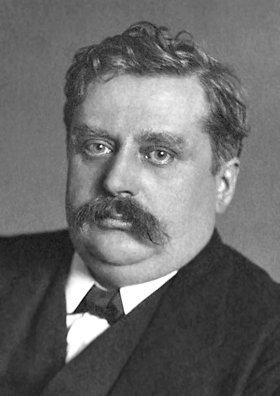
\includegraphics[width=\linewidth]{images/book3/werner.jpg}
\end{minipage}\hfill
\begin{minipage}[t]{0.74\linewidth}
\vspace{0pt}
आल्फ़्रेड वर्नर ने 1893 में प्रस्तावित किया कि किसी धातु की, उसकी संयोजकता के अतिरिक्त, एक
उपसहसंयोजन संख्या होती है, अर्थात् उसके चारों ओर सीधे बँधे समूहों की संख्या, और कोबाल्ट(III)
छह समूहों को एक अष्टफलक के कोनों पर रखता है। फिर उन्होंने पूर्वानुमान लगाया कि हर सूत्र के कितने समावयवी
होने चाहिए और बीस वर्ष उन्हें बनाने में लगाए; 1911 में उन्होंने एक
कोबाल्ट संकुल को उसके दोनों प्रतिबिंबरूपों में वियोजित किया, यह सिद्ध करते हुए कि किरैलता के लिए
कार्बन परमाणु आवश्यक नहीं। उन्हें 1913 में रसायन का नोबेल पुरस्कार मिला। (चित्र: ले प्री
नोबेल, 1914, सार्वजनिक अधिकार-क्षेत्र, विकिमीडिया कॉमन्स।)
\end{minipage}
\end{history}

\section{अभ्यास}

\begin{exercise}[$\star$]\label{exo:b2:coordination-complexes:1}
\ce{Ti^3+}, \ce{V^3+}, \ce{Cr^3+}, \ce{Mn^2+}, \ce{Fe^3+},
\ce{Co^2+}, \ce{Ni^2+} और \ce{Zn^2+} का $d^n$ विन्यास दीजिए।
\end{exercise}

\begin{exercise}[$\star$]\label{exo:b2:coordination-complexes:2}
जल, एथेन-1,2-डाइऐमीन, एथेनडाइओएट आयन, ईडीटीए और
थायोसायनेट आयन की \omterm{def:b2:coordination-complexes:denticity}{दंतुरता} दीजिए, और बताइए कि कौन-सा उभयदंतुर है।
\end{exercise}

\begin{exercise}[$\star$]\label{exo:b2:coordination-complexes:3}
\ce{[Cu(NH3)4]SO4}, \ce{K3[Fe(CN)6]}, \ce{[CoCl2(NH3)4]Cl} और
\ce{[Ni(CO)4]} के नाम लिखिए।
\end{exercise}

\begin{exercise}[$\star$]\label{exo:b2:coordination-complexes:4}
\ce{[Ag(NH3)2]+}, \ce{[CoCl4]^2-}, \ce{[PtCl4]^2-} और
\ce{[Fe(H2O)6]^2+} की ज्यामिति का पूर्वानुमान कीजिए।
\end{exercise}

\begin{exercise}[$\star\star$]\label{exo:b2:coordination-complexes:5}
वर्ग समतलीय \ce{[PtCl2(NH3)2]} के कितने समावयवी हैं? उन्हें खींचिए। (उनमें से एक,
सिसप्लैटिन, कैंसर-रोधी औषधि है।)
\end{exercise}

\begin{exercise}[$\star\star$]\label{exo:b2:coordination-complexes:6}
\ce{Cr(CO)6}, \ce{Fe(CO)5}, \ce{Ni(CO)4},
\ce{V(CO)6} और \ce{Mn2(CO)10} के संयोजकता इलेक्ट्रॉन गिनिए। कौन-सा नियम तोड़ता है, और वह कैसा व्यवहार करता है?
\end{exercise}

\begin{exercise}[$\star\star$]\label{exo:b2:coordination-complexes:7}
फ़ेरोसीन और कोबाल्टोसीन \ce{Co(C5H5)2} के संयोजकता इलेक्ट्रॉन गिनिए। किसका
आसानी से ऑक्सीकरण होता है, और किसमें?
\end{exercise}

\begin{exercise}[$\star\star$]\label{exo:b2:coordination-complexes:8}
ईडीटीए के निकेल(II) संकुल का $\log_{10}K = 20.5$ है, जो उन संकुलों से कहीं ऊपर है जिनमें
निकेल छह अलग-अलग नाइट्रोजन या ऑक्सीजन दाताओं से बँधता है। इस कीलेट प्रभाव को
उन कणों की संख्या के आधार पर समझाइए जो कीलेट द्वारा जल के छह
अणुओं को प्रतिस्थापित करने पर मुक्त होते हैं।
% ledger: logb:Ni-edta
\end{exercise}

\begin{exercise}[$\star\star$]\label{exo:b2:coordination-complexes:9}
\ce{[Co(NO2)(NH3)5]^2+} के दोनों \omterm{def:b2:coordination-complexes:isomers}{बंधनी समावयवी} खींचिए।
\end{exercise}

\begin{exercise}[$\star\star\star$]\label{exo:b2:coordination-complexes:10}
\ce{[CoCl2(en)2]+} के कितने त्रिविम समावयवी हैं? कौन-से किरैल हैं?
\end{exercise}

\begin{exercise}[$\star\star\star$]\label{exo:b2:coordination-complexes:11}
$\mathrm{MA_4B_2}$ के लिए छह लिगैंडों के समतलीय षट्भुज और त्रिकोणीय
प्रिज़्म द्वारा पूर्वानुमित समावयवी गिनिए, और समझाइए कि पाए गए समावयवियों की संख्या
ज्यामितियों के बीच निर्णय कैसे करती है।
\end{exercise}

\begin{exercise}[$\star\star\star$]\label{exo:b2:coordination-complexes:12}
\ce{[RhCl(PPh3)3]} और \ce{[IrH(CO)(PPh3)3]} के संयोजकता इलेक्ट्रॉन गिनिए
(\ce{PPh3} दो-इलेक्ट्रॉन दाता, \ce{H-} हाइड्राइड के रूप में)। कौन-सा दो और
लिगैंड ग्रहण कर सकता है?
\end{exercise}

\section{समस्या: वर्नर के कोबाल्ट ऐम्मीन}

\begin{problem}[{सप्ताहांत समस्या --- कोबाल्ट(III) क्लोराइड के चार ऐम्मीन और उनके द्वारा
मुक्त क्लोराइड, कोष्ठकों के साथ उनके सूत्र, टेट्राऐम्मीन के दोनों समावयवी और वे
ज्यामिति के बारे में क्या सिद्ध करते हैं, और किसी त्रिस-कीलेट की प्रकाशिक सक्रियता}]
\label{pb:b2:coordination-complexes:1}
आँकड़े: चार यौगिक, A \ce{CoCl3.6NH3} (नारंगी-पीला), B \ce{CoCl3.5NH3}
(बैंगनी-लाल), C और D \ce{CoCl3.4NH3} (हरा और बैंगनी)। सिल्वर नाइट्रेट के आधिक्य के साथ
A का एक मोल 3 mol \ce{AgCl} अवक्षेपित करता है, B 2 mol, C और D प्रत्येक 1 mol। मोलर
चालकताएँ प्रति सूत्र इकाई 4, 3, 2 और 2 आयन दर्शाती हैं।

\medskip
\noindent\textbf{भाग I --- क्लोराइड और आयन।}
\begin{enumerate}
  \item कौन-से क्लोराइड सिल्वर आयनों से तुरंत अभिक्रिया करते हैं?
  \item हर यौगिक में कितने क्लोराइड कोबाल्ट से बँधे हैं?
  \item आयनों की संख्याओं को चालकताओं से मिलाकर जाँचिए।
  \item चारों में कोबाल्ट की ऑक्सीकरण संख्या क्या है?
  \item उसका $d^n$ विन्यास क्या है?
  \item हर यौगिक में कोबाल्ट कुल कितने लिगैंड रखता है?
\end{enumerate}

\medskip
\noindent\textbf{भाग II --- सूत्र और नाम।}
\begin{enumerate}[resume]
  \item A, B, C और D को वर्ग कोष्ठकों के साथ लिखिए।
  \item A और B के नाम लिखिए।
  \item C और D के धनायन का नाम लिखिए।
  \item C और D किस प्रकार के समावयवी हैं?
  \item यौगिक \ce{CoCl3.3NH3} क्या होगा, और वह कितने आयन देगा?
  \item अष्टफलक में उस यौगिक के कितने समावयवी होंगे?
\end{enumerate}

\medskip
\noindent\textbf{भाग III --- ज्यामिति।}
\begin{enumerate}[resume]
  \item अष्टफलक में cis और trans \ce{[CoCl2(NH3)4]+} खींचिए।
  \item समतलीय षट्भुज के कोनों पर छह लिगैंडों के लिए पूर्वानुमित
        \ce{[CoCl2(NH3)4]+} के समावयवी गिनिए।
  \item त्रिकोणीय प्रिज़्म के लिए पूर्वानुमित समावयवी गिनिए।
  \item वर्नर को कभी दो से अधिक नहीं मिले। इससे क्या सिद्ध होता है?
  \item क्या प्रमाण पूर्ण है? तीसरे समावयवी का क्या अर्थ होता?
  \item C और D में से कौन-सा cis है, यह जानते हुए कि cis समावयवी को एथेनडाइओएट के साथ
        कीलेट में बदला जा सकता है और trans को नहीं?
\end{enumerate}

\medskip
\noindent\textbf{भाग IV --- प्रकाशिक सक्रियता।}
\begin{enumerate}[resume]
  \item \ce{[Co(en)3]^3+} खींचिए।
  \item क्या इसका कोई दर्पण तल है? कोई प्रतिलोमन केंद्र?
  \item इसके कितने त्रिविम समावयवी हैं?
  \item ऐसे किसी धनायन का प्रतिबिंबरूपों में वियोजन क्या सिद्ध करता है?
  \item क्या \ce{[CoCl2(en)2]+} अपने cis रूप में किरैल है? अपने trans रूप में?
  \item बिल्कुल कार्बन-रहित किसी संकुल का वर्नर द्वारा किया गया वियोजन महत्त्वपूर्ण क्यों था?
  \item अष्टफलक द्वारा, और समतलीय षट्भुज तथा त्रिकोणीय प्रिज़्म द्वारा पूर्वानुमित
        \ce{[CoCl2(NH3)4]+} के समावयवियों की संख्या बताइए।
\end{enumerate}
\end{problem}
